% abtex2-modelo-artigo.tex, v-1.9.2 laurocesar
% Copyright 2012-2014 by abnTeX2 group at http://abntex2.googlecode.com/ 
%

% ------------------------------------------------------------------------
% ------------------------------------------------------------------------
% abnTeX2: Modelo de Artigo Acadêmico em conformidade com
% ABNT NBR 6022:2003: Informação e documentação - Artigo em publicação 
% periódica científica impressa - Apresentação
% ------------------------------------------------------------------------
% ------------------------------------------------------------------------

\documentclass[
% -- opções da classe memoir --
article,			% indica que é um artigo acadêmico
11pt,				% tamanho da fonte
oneside,			% para impressão apenas no verso. Oposto a twoside
a4paper,			% tamanho do papel. 
% -- opções da classe abntex2 --
%chapter=TITLE,		% títulos de capítulos convertidos em letras maiúsculas
%section=TITLE,		% títulos de seções convertidos em letras maiúsculas
%subsection=TITLE,	% títulos de subseções convertidos em letras maiúsculas
%subsubsection=TITLE % títulos de subsubseções convertidos em letras maiúsculas
% -- opções do pacote babel --
english,			% idioma adicional para hifenização
brazil,				% o último idioma é o principal do documento
sumario=tradicional
]{abntex2}


% ---
% PACOTES
% ---

% ---
% Pacotes fundamentais 
% ---
\usepackage{lmodern}			% Usa a fonte Latin Modern
\usepackage[T1]{fontenc}		% Selecao de codigos de fonte.
\usepackage[utf8]{inputenc}		% Codificacao do documento (conversão automática dos acentos)
\usepackage{indentfirst}		% Indenta o primeiro parágrafo de cada seção.
\usepackage{nomencl} 			% Lista de simbolos
\usepackage{color}				% Controle das cores
\usepackage{graphicx}			% Inclusão de gráficos
\usepackage{microtype} 			% para melhorias de justificação
% ---

% ---
% Pacotes adicionais, usados apenas no âmbito do Modelo Canônico do abnteX2
% ---
\usepackage{lipsum}				% para geração de dummy text
% ---

% ---
% Pacotes de citações
% ---
\usepackage[brazilian,hyperpageref]{backref}	 % Paginas com as citações na bibl
\usepackage[alf]{abntex2cite}	% Citações padrão ABNT
% ---

% ---
% Configurações do pacote backref
% Usado sem a opção hyperpageref de backref
\renewcommand{\backrefpagesname}{Citado na(s) página(s):~}
% Texto padrão antes do número das páginas
\renewcommand{\backref}{}


% ---
% Informações de dados para CAPA e FOLHA DE ROSTO
% ---
\titulo{INE5429 - Segurança de Computadores}
\autor{Mateus Rissi \and Rodrigo Pedro Marques}
\local{Florianópolis}
\data{Março de 2017}
% ---

% ---
% Configurações de aparência do PDF final

% alterando o aspecto da cor azul
\definecolor{blue}{RGB}{41,5,195}

% informações do PDF
\makeatletter
\hypersetup{
	%pagebackref=true,
	pdftitle={\@title}, 
	pdfauthor={\@author},
	pdfsubject={Modelo de artigo científico com abnTeX2},
	pdfcreator={LaTeX with abnTeX2},
	pdfkeywords={abnt}{latex}{abntex}{abntex2}{atigo científico}, 
	colorlinks=true,       		% false: boxed links; true: colored links
	linkcolor=blue,          	% color of internal links
	citecolor=blue,        		% color of links to bibliography
	filecolor=magenta,      		% color of file links
	urlcolor=blue,
	bookmarksdepth=4
}
\makeatother
% --- 

% ---
% compila o indice
% ---
\makeindex
% ---

% ---
% Altera as margens padrões
% ---
\setlrmarginsandblock{3cm}{3cm}{*}
\setulmarginsandblock{3cm}{3cm}{*}
\checkandfixthelayout
% ---

% --- 
% Espaçamentos entre linhas e parágrafos 
% --- 

% O tamanho do parágrafo é dado por:
\setlength{\parindent}{1.3cm}

% Controle do espaçamento entre um parágrafo e outro:
\setlength{\parskip}{0.2cm}  % tente também \onelineskip

% Espaçamento simples
\SingleSpacing

% ----
% Início do documento
% ----
\begin{document}
	
	% Retira espaço extra obsoleto entre as frases.
	\frenchspacing 
	
	% ----------------------------------------------------------
	% ELEMENTOS PRÉ-TEXTUAIS
	% ----------------------------------------------------------
	
	%---
	%
	% Se desejar escrever o artigo em duas colunas, descomente a linha abaixo
	% e a linha com o texto ``FIM DE ARTIGO EM DUAS COLUNAS''.
	% \twocolumn[    		% INICIO DE ARTIGO EM DUAS COLUNAS
	%
	%---
	% página de titulo
	\maketitle
	
	% resumo em português
	
	% ]  				% FIM DE ARTIGO EM DUAS COLUNAS
	% ---
	
	% ----------------------------------------------------------
	% ELEMENTOS TEXTUAIS
	% ----------------------------------------------------------
	\textual
	
	% ----------------------------------------------------------
	% Introdução
	% ----------------------------------------------------------
	\section*{Implementação dos algoritmo Cifra de Cesar, \textit{PlayFair} e Viginère}
	
	\section{Cifra de César}
			Cifra de César é um tipo de cifra de substituição onde cada letra do texto é substituída por outra letra do mesmo alfabeto, porém, esta outra letra está em uma posição abaixo dela em um número fixo de vezes.
			
			
			\begin{figure} [!h]
			\centering
			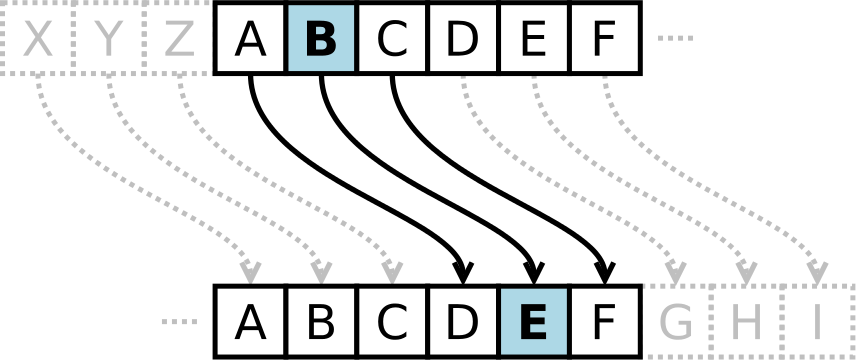
\includegraphics[width=0.7\linewidth]{Imagens/cesar}
			\caption{Exemplo de Cifra de César com chave igual a 3.}
			\label{fig:cesar}
			\end{figure}
			
			Na figura \ref{fig:cesar}, onde a chave – que indica quantas casas o alfabeto será movido – é igual a 3,  é demonstrado que a letra B corresponde a letra E.
			
			A cifra tem esse nome em homenagem a Julio César que, segundo Suetónio, a usava com uma troca de três posições para proteger mensagens de significado militar. Por exemplo:
			
			\textbf{Alfabeto Normal:}  ABCDEFGHIJKLMNOPQRSTUVWXYZ
			
			\textbf{Alfabeto Cifrado:}  DEFGHIJKLMNOPQRSTUVWXYZABC
			
			Assim, a aplicação deste método em uma mensagem como ``\textit{a ligeira raposa marrom saltou sobre o cachorro cansado}'', resultaria na seguinte mensagem cifrada: ``\textit{D OLJHLUD UDSRVD PDUURP VDOWRX VREUH R FDFKRUUR FDQVDGR}''.
			
			\subsubsection*{Decifrando}
				A Cifra de César é uma das mais simples e conhecidas técnicas de criptografia e, como todas as cifras de substituição monoalfabéticas, a cifra de César é facilmente decifrada e na prática não oferece essencialmente nenhuma segurança na comunicação. Para decifrar a mensagem cifrada duas situações podem ser consideradas:
				\begin{enumerate}
					\item Um interceptor conhece (ou adivinha) que algum tipo de cifra de substituição simples foi utilizado, mas não especificamente que é uma Cifra de César.
					\item Um interceptor sabe que uma cifra de César foi usada, mas não sabe o valor da troca.
				\end{enumerate}

				No primeiro caso, a cifra pode ser decifrada usando análise de frequência ou verificando os padrões de palavras. No segundo caso é ainda mais simples, pois existem apenas um número limitado de rotações possíveis (26 no alfabeto português brasileiro).
	
	\section{\textit{PlayFair}}
		A Cifra \textit{Playfair} usa uma tabela de 5 por 5 contendo uma palavra ou até uma frase chave. Memorizar a chave e as 4 simples regras são tudo o que é necessário para montar a tabela e usar a cifra.
		
		Primeiramente, para criar a tabela é necessário completar os espaços na tabela com as letras da palavra chave – sem letras repetidas – e então completar o resto da tabela com as letras do alfabeto em ordem. Como só há 25 espaços na tabela, métodos como omitir a letra Q ou unir a letra I e J no mesmo espaço são comumente utilizados.
		
		Para cifrar uma mensagem devemos quebra-la em digramas – grupos de 2 letras – como, por exemplo, ``HelloWorld'' vira ``HE LL OW OR LD'', e então mapear na tabela. É necessário que sejam digramas, então numa palavra de número ímpar devemos adicionar algum outro caractere para completar o par. Agora pense no digrama como cantos opostos de um retângulo dentro da tabela e então aplique as 4 regras seguintes, em ordem, para cada par da mensagem:
		
		\begin{enumerate}
			\item Se as letras do par são iguais (ou há apenas 1 letra), adicione um X após a primeira letra. Cifre o novo par e continue.
			\item Se as letras do par estão na mesma linha, substitua elas pelas letras que estão imediatamente a sua direita (mudando para a esquerda se a letra no par original estava do lado direito).
			\item Se as letras aparecem na mesma coluna, substitua elas pelas letras que estão imediatamente abaixo (mudando para cima se a letra no par original estava no final da coluna).
			\item Se as letras do par não estão na mesma linha ou coluna, substitua elas pelas letras que estão na mesma linha mas que representam o outro par de cantos do retângulo definido pelo par original. A ordem importa – a primeira letra do par cifrado deve ser a que estava na mesma linha que a primeira letra do par original.
		\end{enumerate}
	
		Para decifrar o texto use o inverso das 3 últimas regras e a regra 1 como está (só que retirando qualquer ``X'' extra que não faz sentido na mensagem final).
		
		
		A figura \ref{fig:playfair} apresenta um exemplo onde a palavra ``\textit{PlayfairExample}'' foi utilizada como palavra chave (letras em vermelho são as que foram omitidas).		
		
		\begin{figure} [!h]
		\centering
		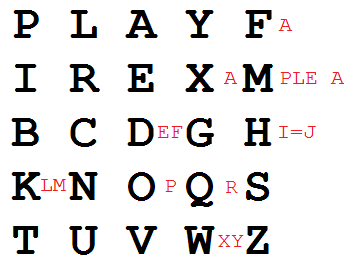
\includegraphics[width=0.5\linewidth]{Imagens/playfair}
		\caption{PlayFairExample}
		\label{fig:playfair}
		\end{figure}
		
		
	\section{Vinegère}
		Esta cifra consiste no uso de várias cifras de César em sequência, com diferentes valores de deslocamento ditados por uma ``palavra-chave''. Para cifrar, é usada uma tabela de alfabetos que consiste no alfabeto escrito 26 vezes em diferentes linhas, cada um deslocado ciclicamente do anterior por uma posição. As 26 linhas correspondem às 26 possíveis cifras de César. Uma palavra é escolhida como ``palavra-chave'', e cada letra desta palavra vai indicar a linha a ser utilizada para cifrar ou decifrar uma letra da mensagem. É possível observar essa tabela na figura \ref{fig:vinegere}.		
		
		\begin{figure}[!h]
			\centering
			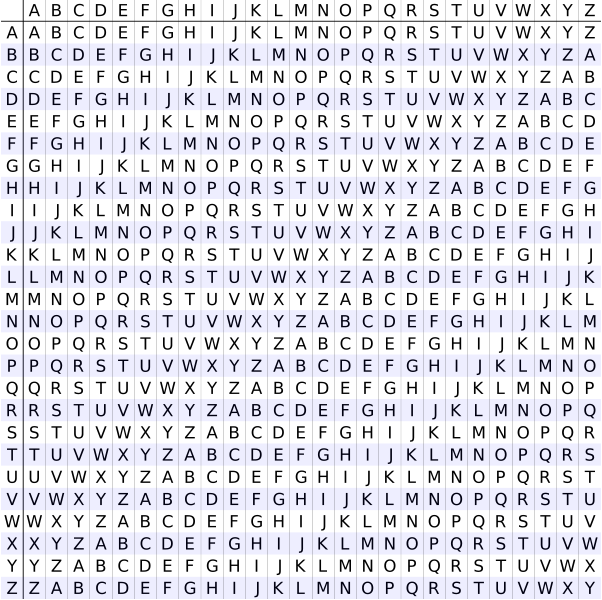
\includegraphics[width=0.7\linewidth]{Imagens/vinegere}
			\caption{Tabela de Vinegère}
			\label{fig:vinegere}
		\end{figure}

		
		Caso queiramos criptografar, por exemplo, a mensagem ``\textit{WEHAVEAMEETINGINTWOMINUTES}'' e a palavra chave é ``\textit{CODEX}'', como mostra a figura \ref{fig:venegere2}, a mensagem resultante será ``\textit{YSKESGOPIBVWQKFPHZSJKBXXBU}''.
			
		\begin{figure} [h!]
			\centering
			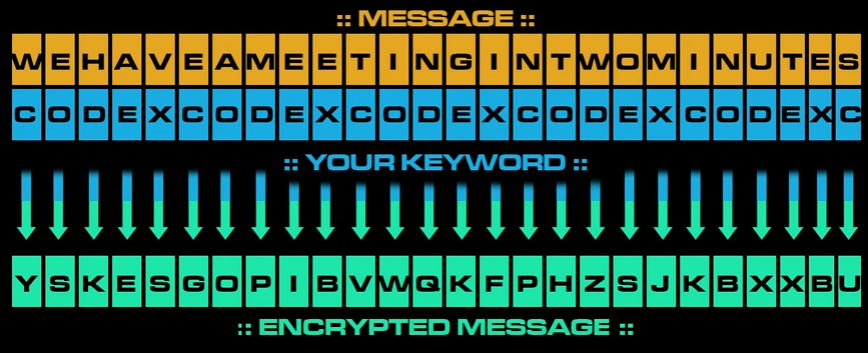
\includegraphics[width=0.7\linewidth]{Imagens/vinegere2.png}
			\caption{Exemplo de criptografia através do método de Vinegère.}
			\label{fig:venegere2}
		\end{figure}
		
		Para decifrar tomamos o caminho inverso, como mostra a figura \ref{fig:vinegere3}.
		
		\begin{figure} [h!]
			\centering
			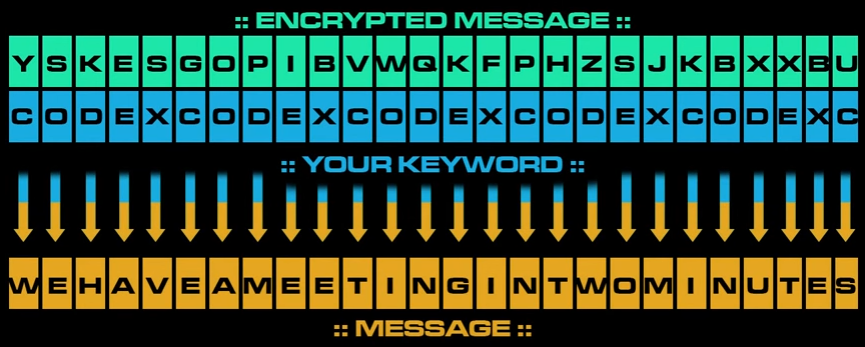
\includegraphics[width=0.7\linewidth]{Imagens/vinegere3.png}
			\caption{Exemplo de decifragem através do método de Vinegère.}
			\label{fig:vinegere3}
		\end{figure}
		
		As cifras polialfabéticas são mais difíceis de quebrar por análise de frequência, mas têm uma fraqueza se a chave é curta e constantemente repetida. Como resultado, palavras comuns como ``de'' vão provavelmente aparecer criptografadas segundo as mesmas letras da chave, levando à descoberta de padrões repetidos no texto.

\end{document}